\documentclass{article}
\usepackage[utf8]{inputenc}
\usepackage{tikz}
\usetikzlibrary{positioning}

\begin{document}

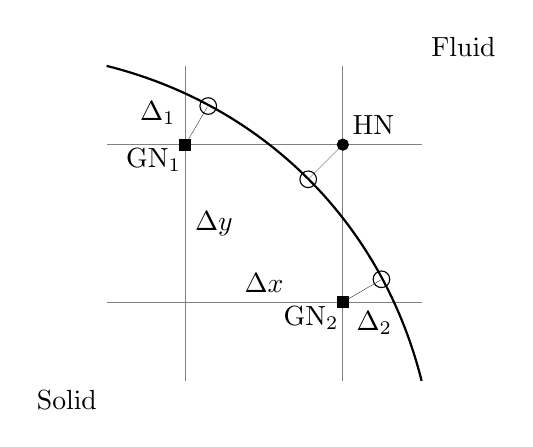
\begin{tikzpicture}
%\draw[step=2cm,gray,very thin] (-2,-2) grid (2,2); %make a grid, this will put a point at 0,0 and I cant figure out how to make it have an offset
\draw[gray, thin] (-2,1) -- (2,1);      %horizontal line
\draw[gray, thin] (-2,-1) -- (2,-1);    %horizontal line
\draw[gray, thin] (-1,2) -- (-1,-2);    %vertical line
\draw[gray, thin] (1,2) -- (1,-2);      %vertical line
 %end point of arc .. streach to these points .. other end point of arc
\draw[black, thick] (-2,2) .. controls (0,1.5) and (1.5,0) .. (2,-2);                                   %body surface
\filldraw [black] (1,1) circle (2pt) node[anchor=south west] {HN};                                      %hybrid node
\draw [black] (0.56,0.56) circle (3pt);                                                                 %hybrid node body intercept
\draw [black, ultra thin] (0.56, 0.56) -- (1,1);                                                        %HN line
\filldraw ([xshift=-2pt,yshift=-2pt]-1,1) rectangle ++(4pt,4pt) node[anchor=north east] {GN$_1$};       %ghost node 1
\draw [black] (-0.71,1.49) circle (3pt);                                                                %ghost node 1 body intercept
\draw [black, ultra thin] (-0.72, 1.48) -- (-1,1);                                                      %GN1 line
\draw [black] (-1,1.4) circle (0pt) node[anchor=east] {$\Delta_1$};                                     %ghost node 1 body intercept label
\filldraw ([xshift=-2pt,yshift=-2pt]1,-1) rectangle ++(4pt,4pt) node[anchor=north east] {GN$_2$};       %ghost node 2
\draw [black] (1.49,-0.71) circle (3pt);                                                                %ghost node 2 body intercept
\draw [black, ultra thin] (1.48, -0.72) -- (1,-1);                                                      %GN2 line
\draw [black] (1.4,-1) circle (0pt) node[anchor=north] {$\Delta_2$};                                    %ghost node 2 body intercept label
\draw [black] (0,-1) circle (0pt) node[anchor=south] {$\Delta x$};                                      %dx label
\draw [black] (-1,0) circle (0pt) node[anchor=west] {$\Delta y$};                                       %dy label
\draw [black] (-2,-2) circle (0pt) node[anchor=north east] {Solid};                                     %Solid label
\draw [black] (2,2) circle (0pt) node[anchor=south west] {Fluid};                                       %Fluid label


\end{tikzpicture}


\end{document}
